\section{Scenario 1}\label{sec:scenario1}
The purpose of this scenario is to simulate 4 controllers in order to compare them using the map in Figure \ref{fig:s1_map}. 

\begin{figure}[H]
	\hfill
	\subfigure[UAS Map Positioning]{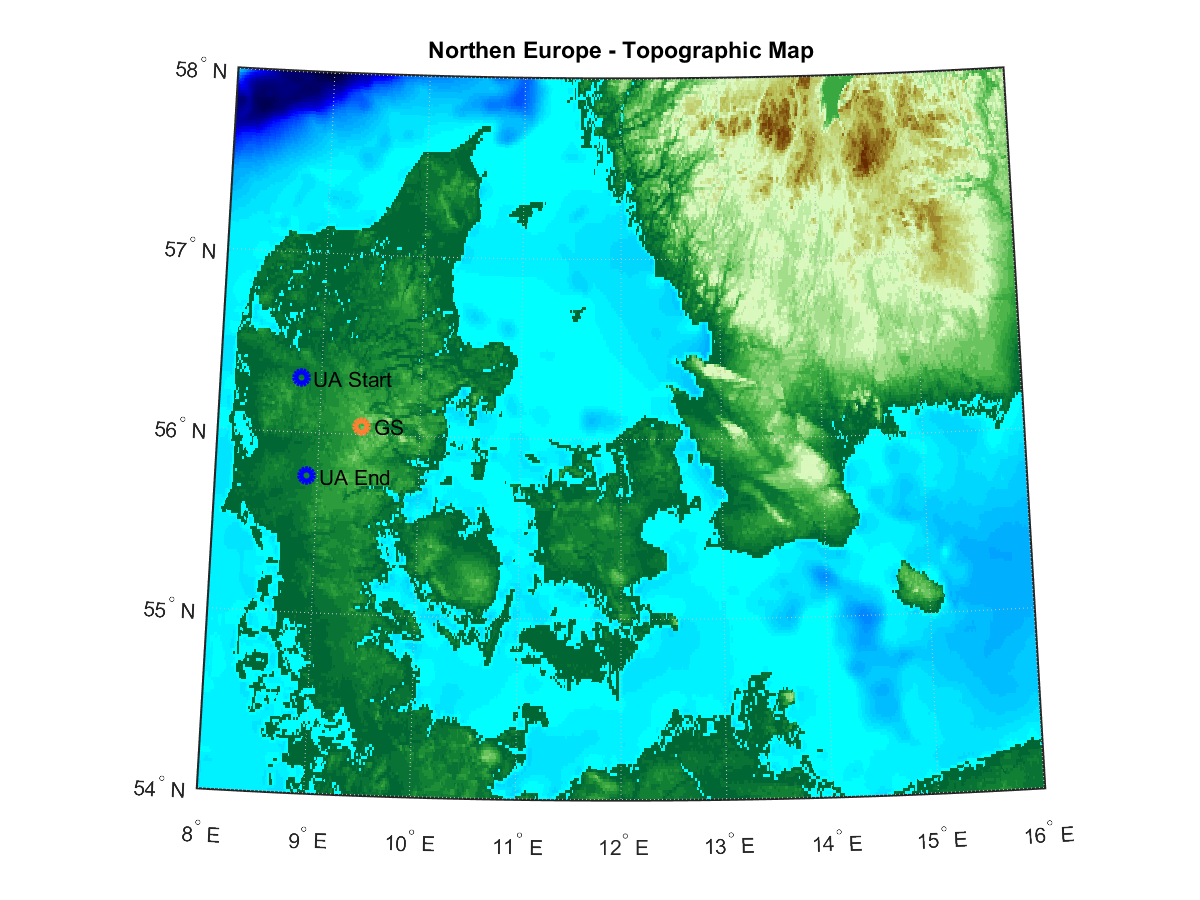
\includegraphics[scale=0.34]{figures/s1_map.png}}
	\hfill
	\subfigure[LOS and Distance]{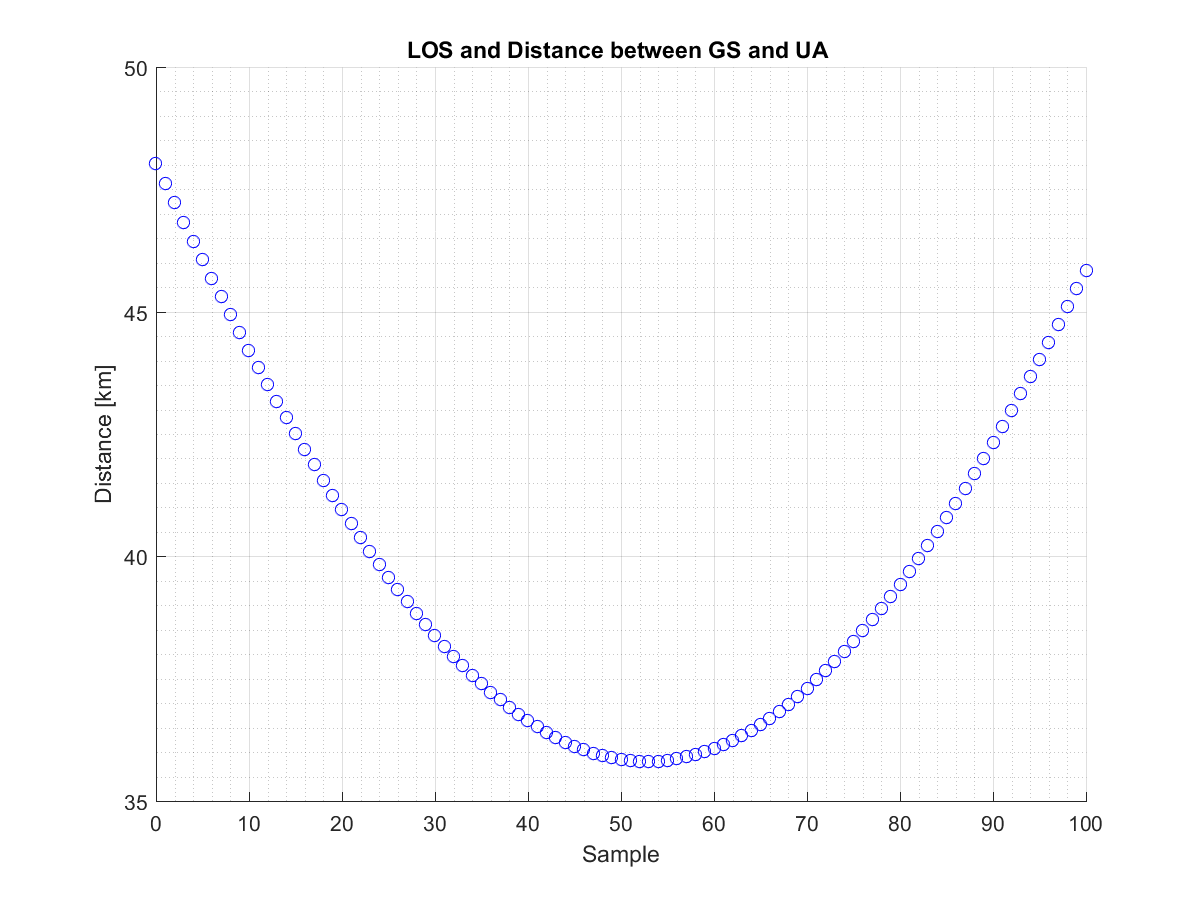
\includegraphics[scale=0.34]{figures/s1_los.png}}
	\hfill
	\caption{Mountain Scenario}
	\label{fig:s1_map}
\end{figure}

\subsection{UA}
In Figure \ref{fig:s1_ua} the angle tracking of the UA antenna can be seen.

\begin{figure}[H]
	\hfill
	\subfigure[P]{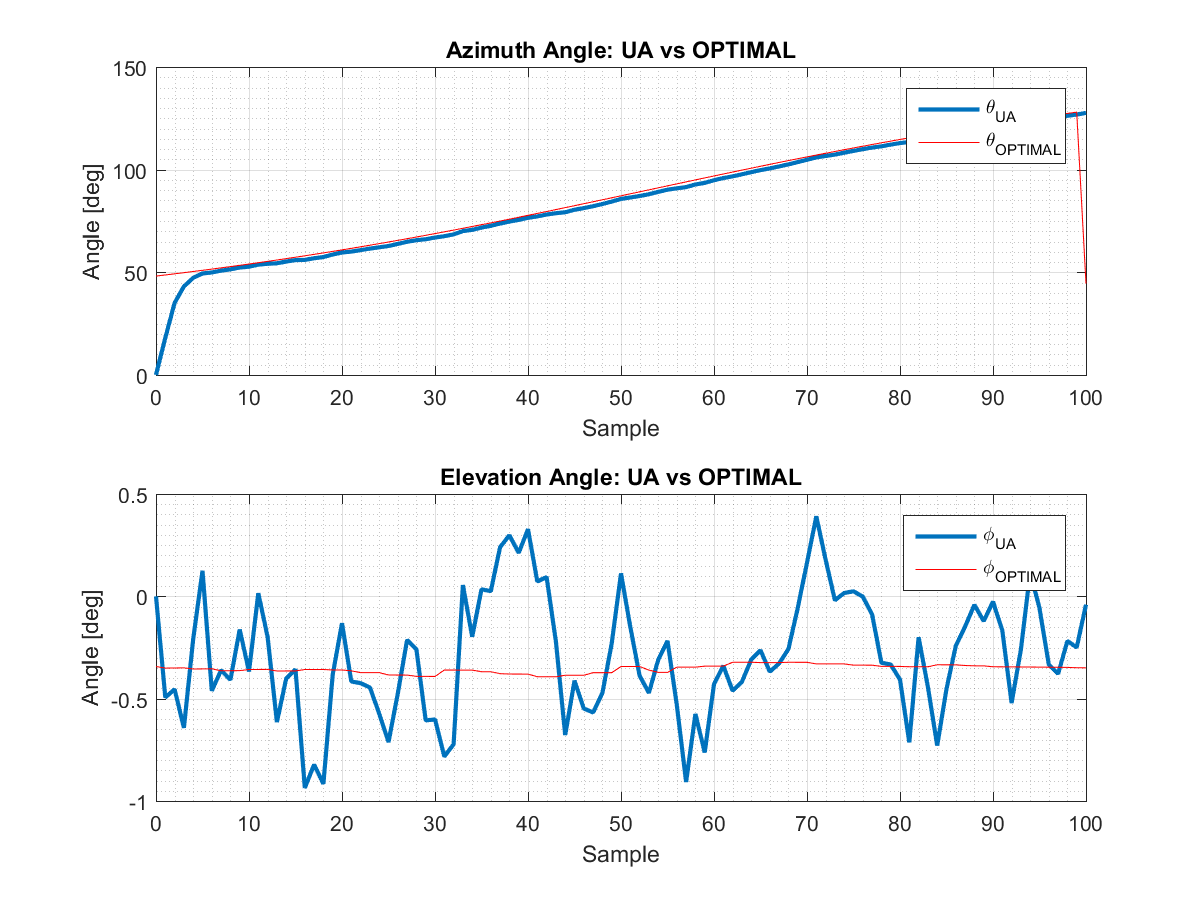
\includegraphics[scale=0.34]{figures/s1_p_ua.png}}
	\hfill
	\subfigure[PI]{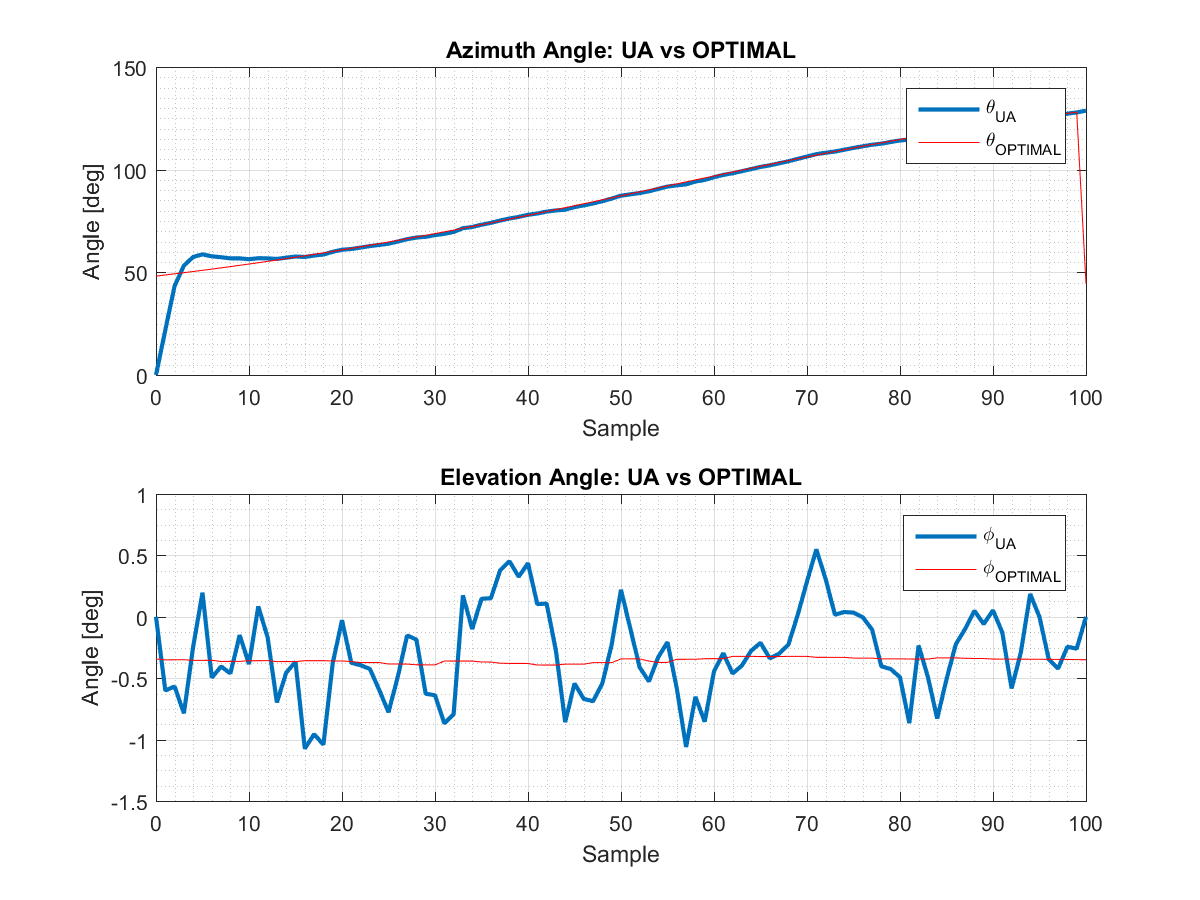
\includegraphics[scale=0.34]{figures/s1_pi_ua.png}}
	\hfill
	\\
	\hfill
	\subfigure[PD]{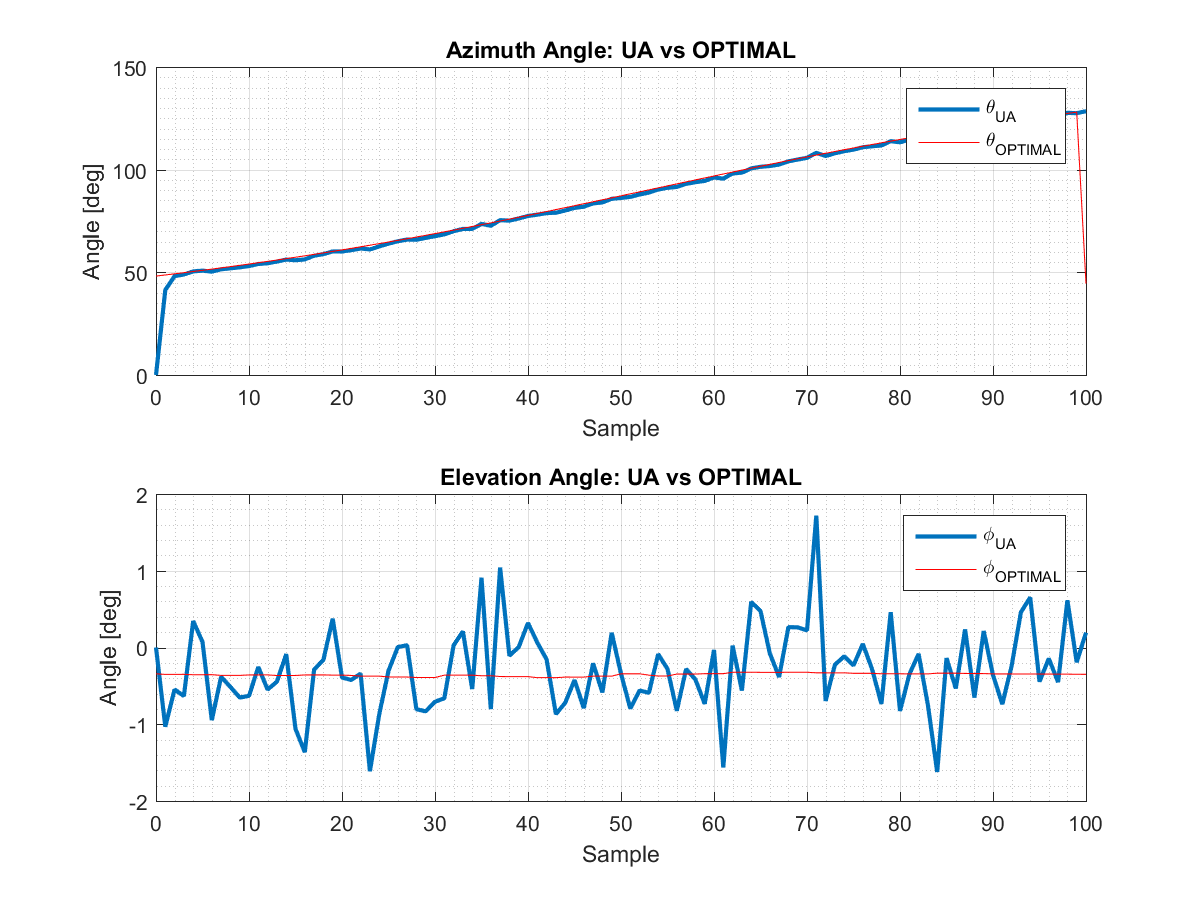
\includegraphics[scale=0.34]{figures/s1_pd_ua.png}}
	\hfill
	\subfigure[PID]{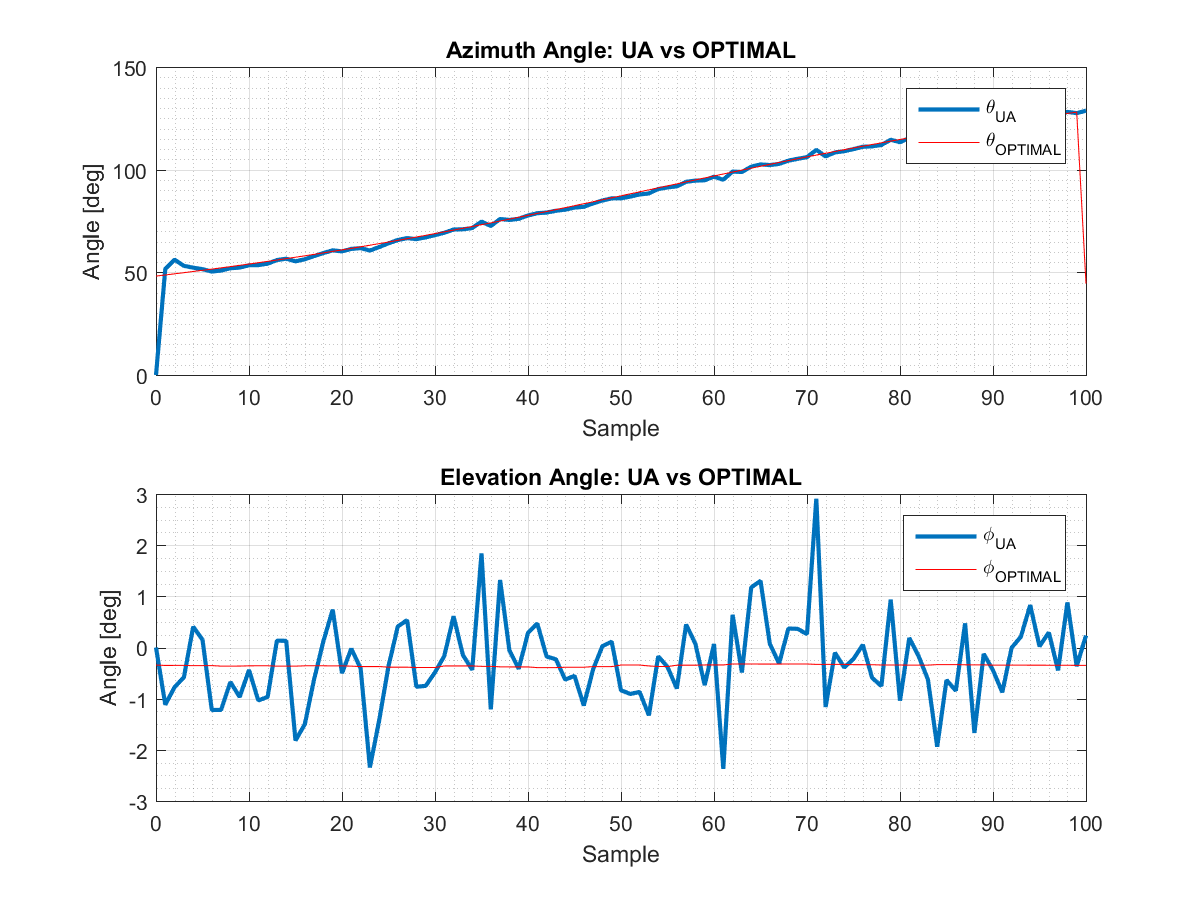
\includegraphics[scale=0.34]{figures/s1_pid_ua.png}}
	\hfill
	\caption{UA Controllers}
	\label{fig:s1_ua}
\end{figure}

\subsection{GS}
In Figure \ref{fig:s2_gs} the angle tracking of the GS antenna can be seen.

\begin{figure}[H]
	\hfill
	\subfigure[P]{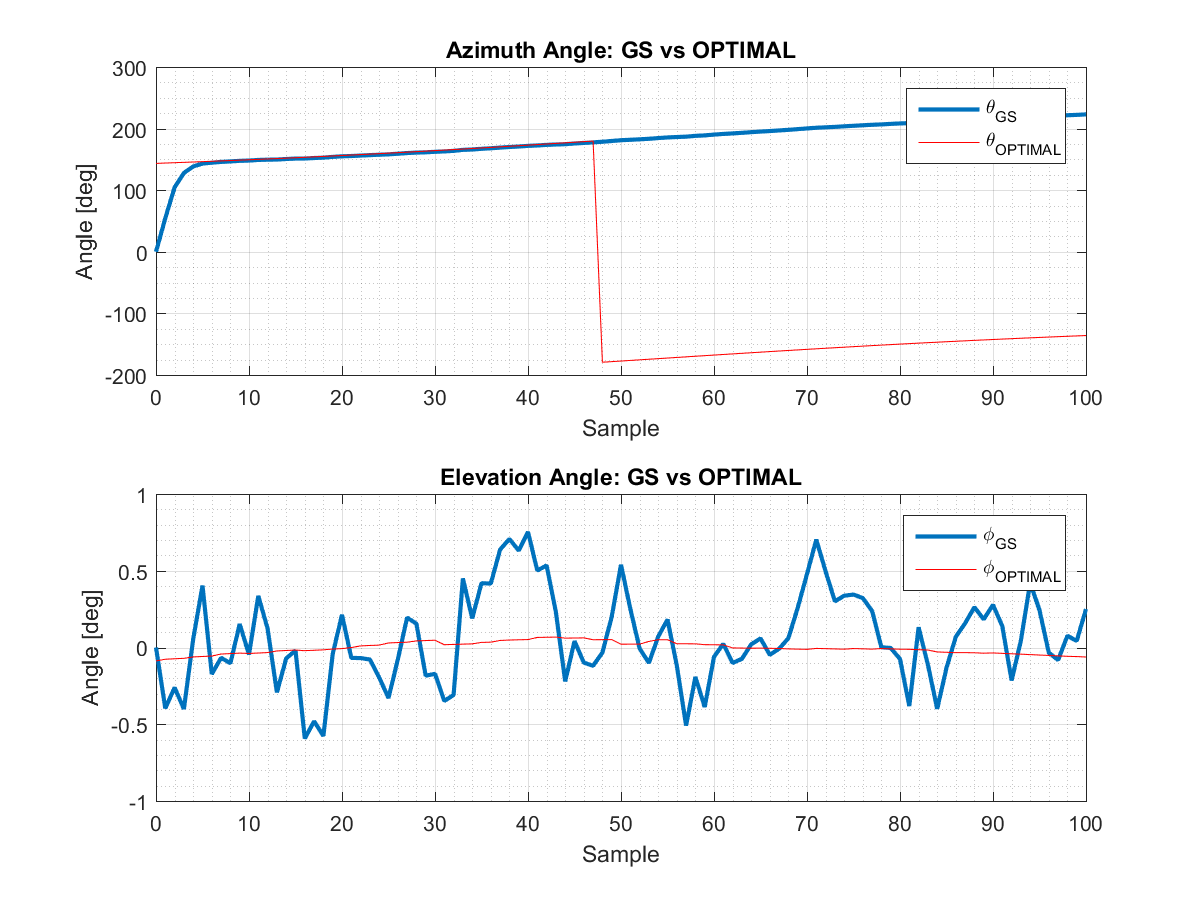
\includegraphics[scale=0.34]{figures/s1_p_gs.png}}
	\hfill
	\subfigure[PI]{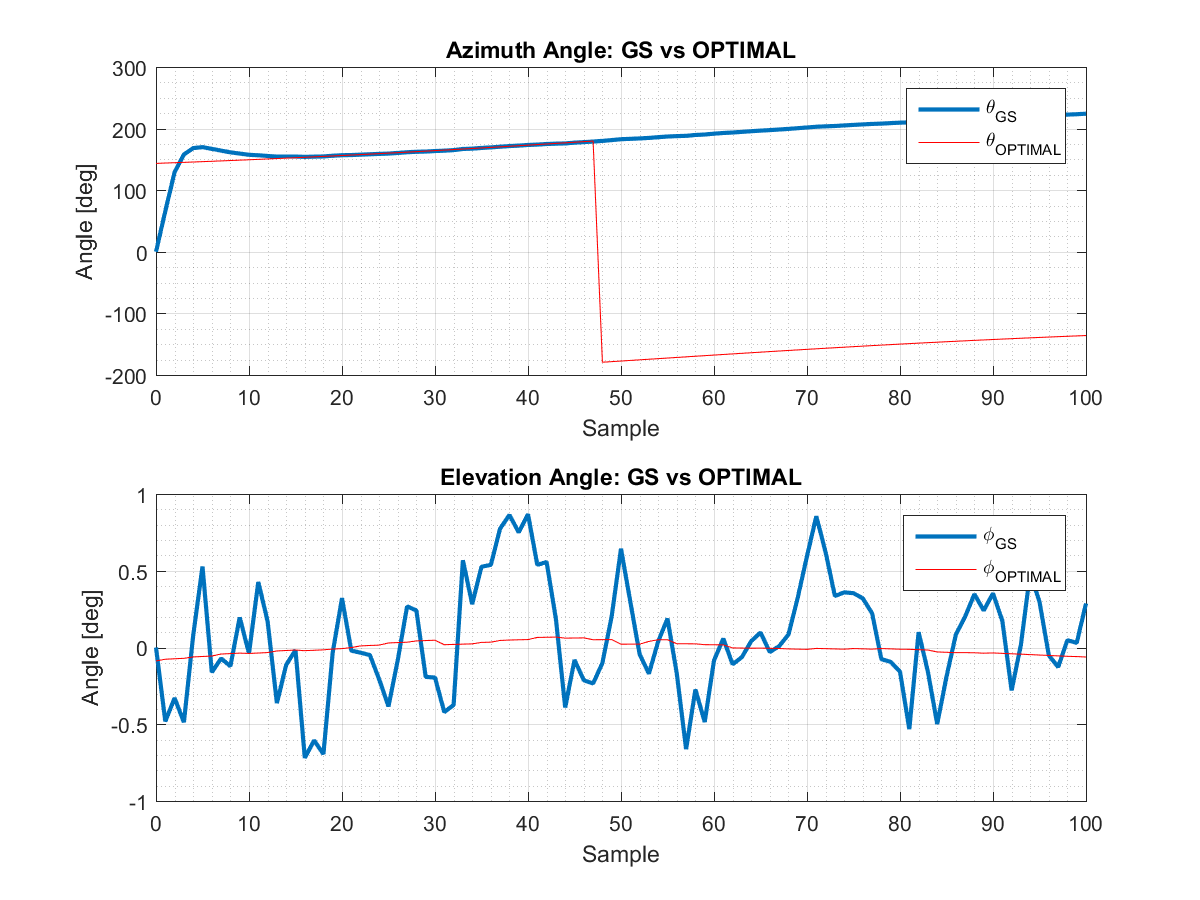
\includegraphics[scale=0.34]{figures/s1_pi_gs.png}}
	\hfill
	\\
	\hfill
	\subfigure[PD]{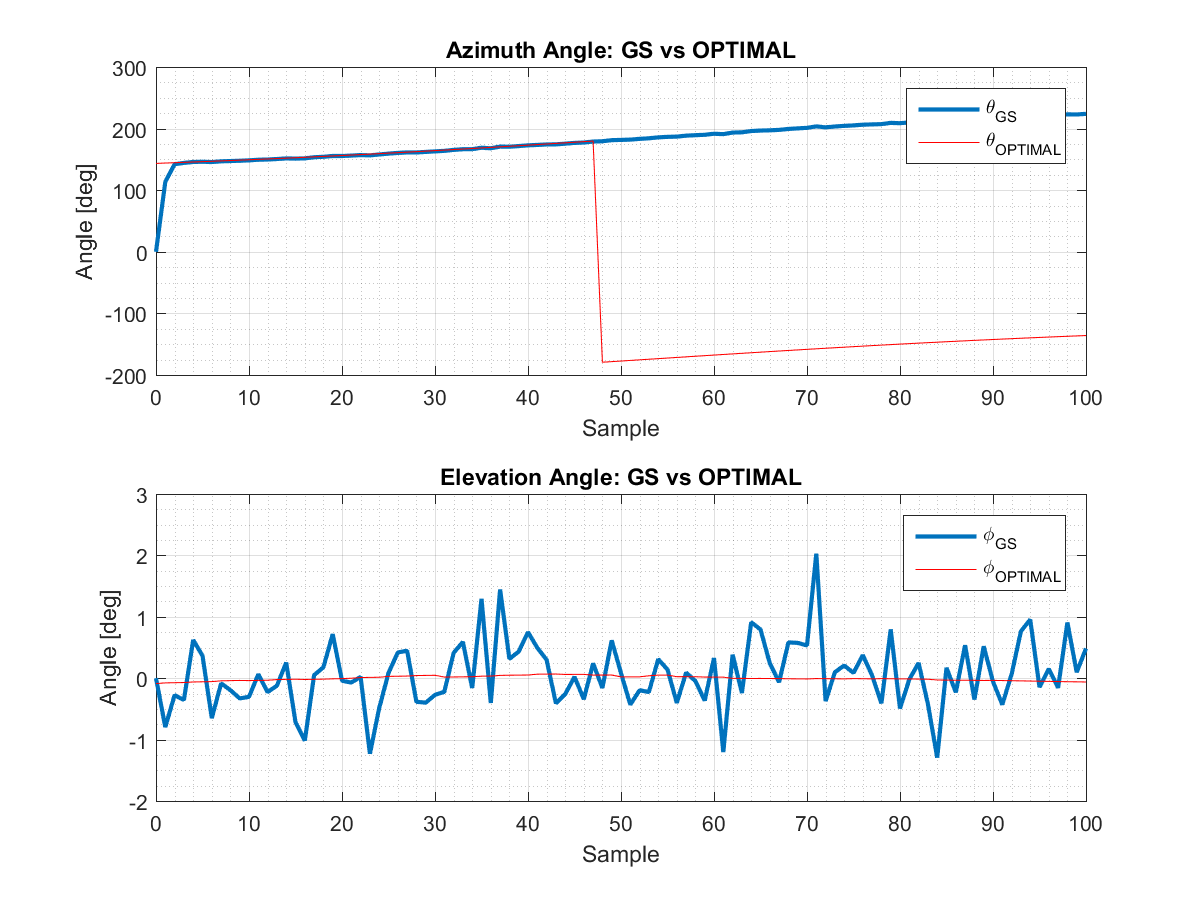
\includegraphics[scale=0.34]{figures/s1_pd_gs.png}}
	\hfill
	\subfigure[PID]{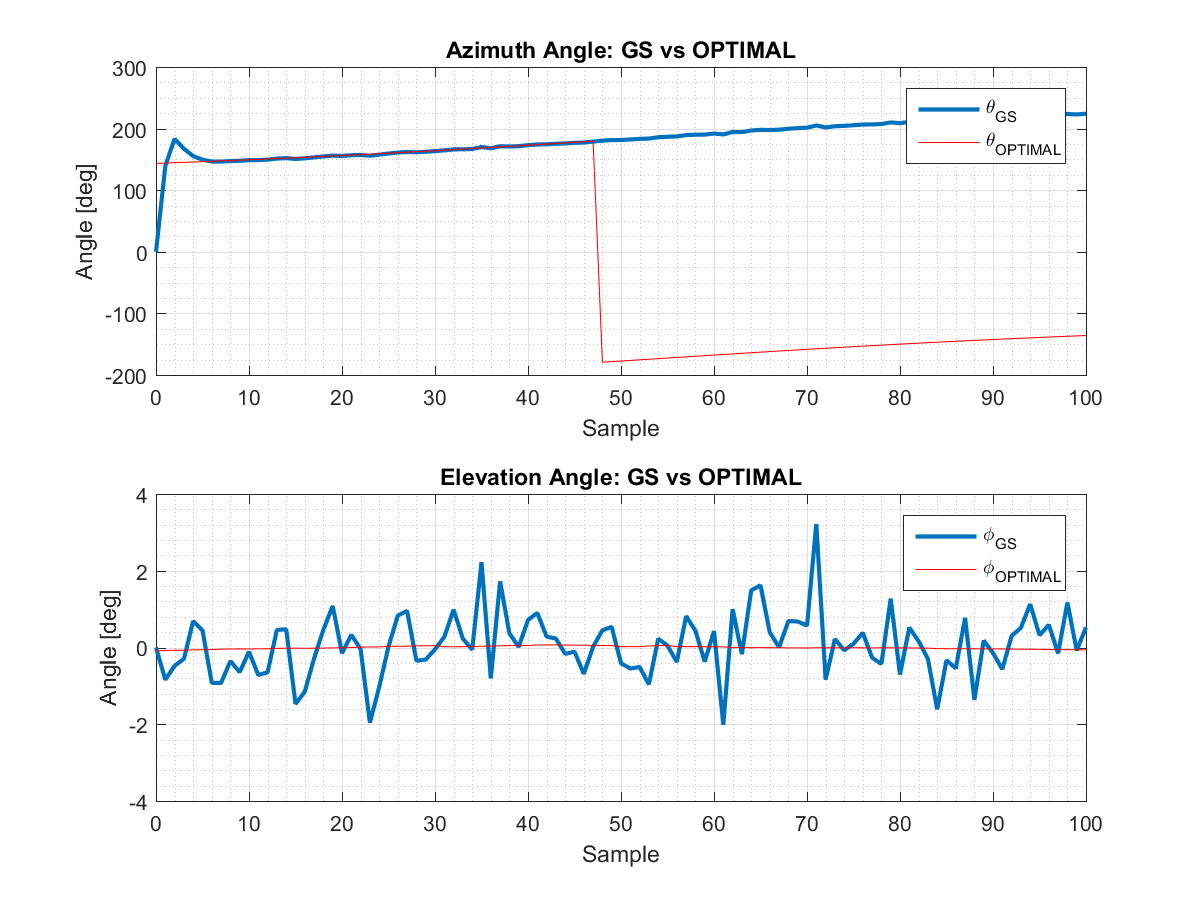
\includegraphics[scale=0.34]{figures/s1_pid_gs.png}}
	\hfill
	\caption{UA Controllers}
	\label{fig:s1_gs}
\end{figure}

\subsection{Power}
In Figure \ref{fig:s2_power} the power at the receiver antenna of the GS antenna can be seen.

\begin{figure}[H]
	\hfill
	\subfigure[P]{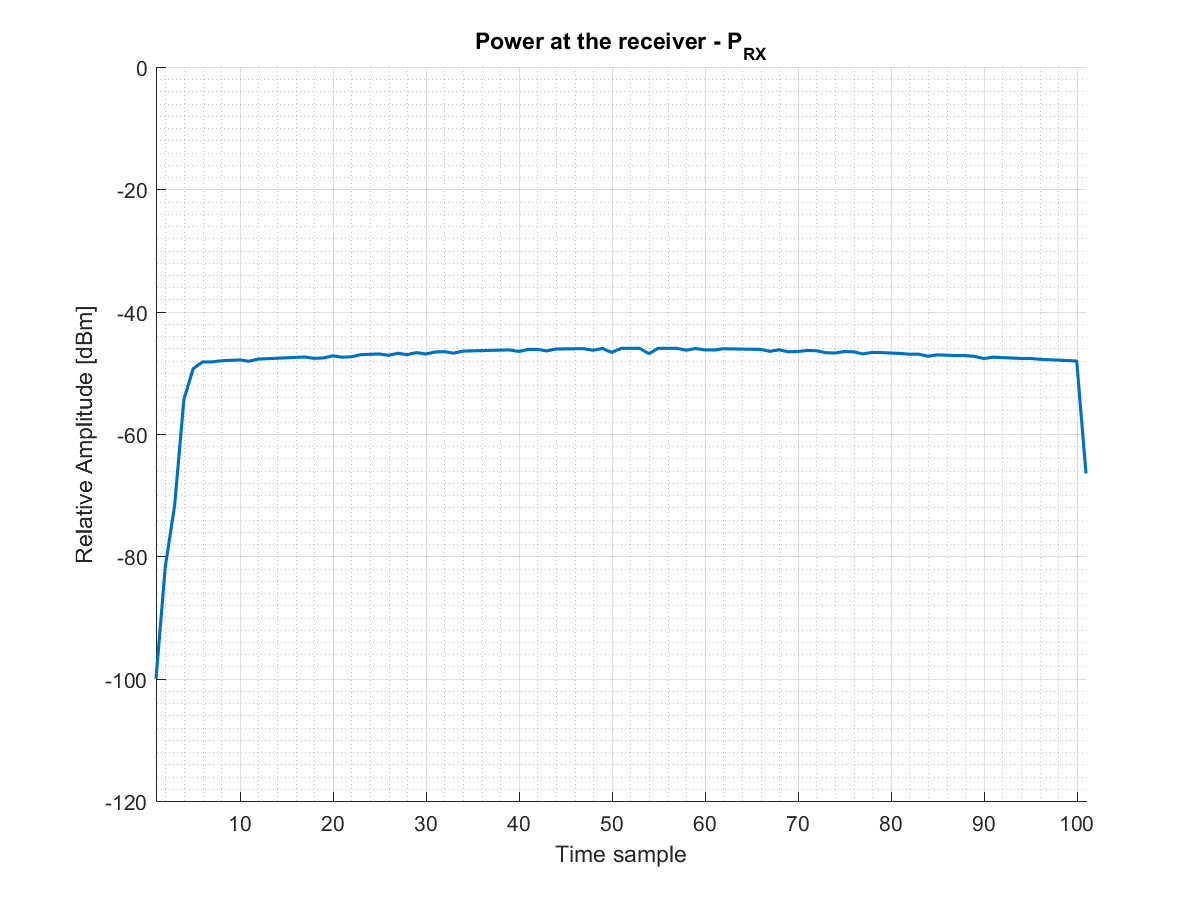
\includegraphics[scale=0.34]{figures/s1_p_power.png}}
	\hfill
	\subfigure[PI]{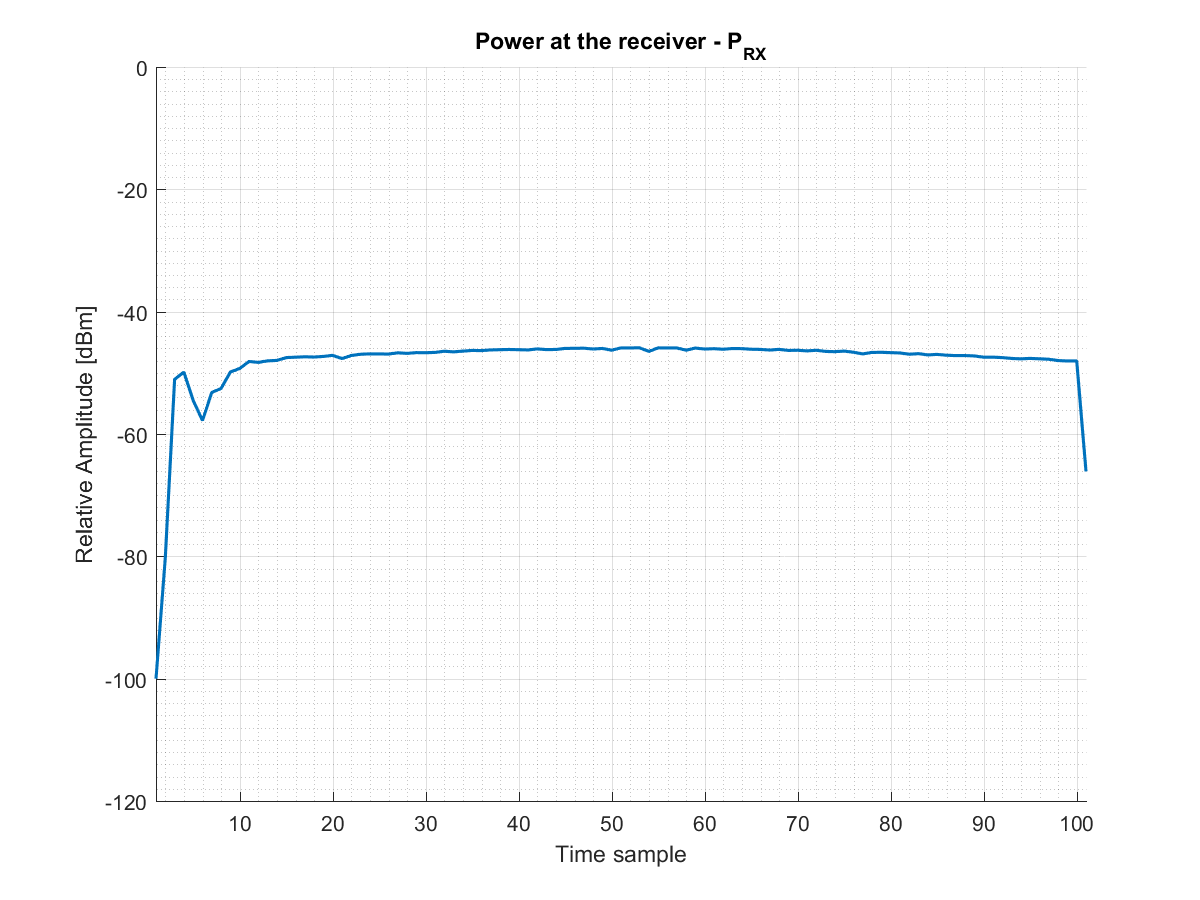
\includegraphics[scale=0.34]{figures/s1_pi_power.png}}
	\hfill
	\\
	\hfill
	\subfigure[PD]{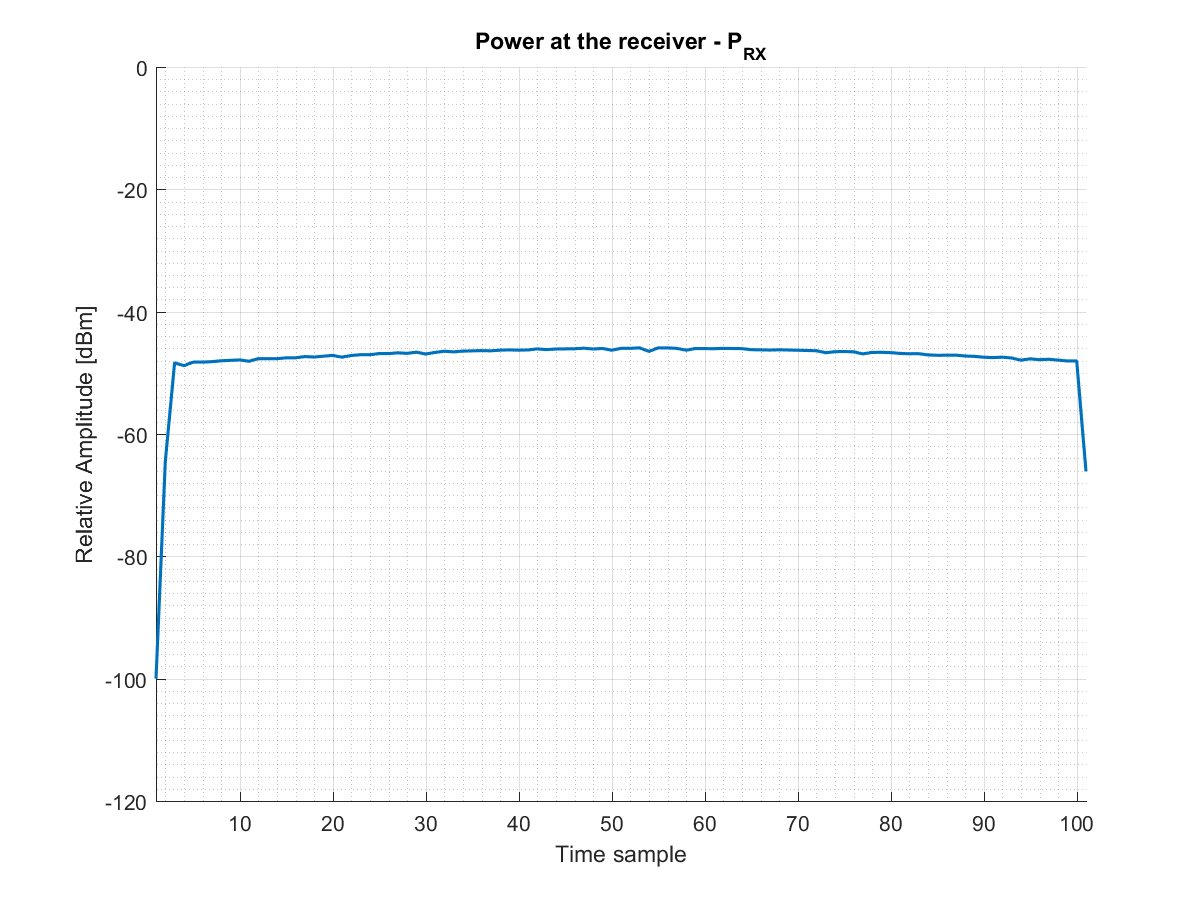
\includegraphics[scale=0.34]{figures/s1_pd_power.png}}
	\hfill
	\subfigure[PID]{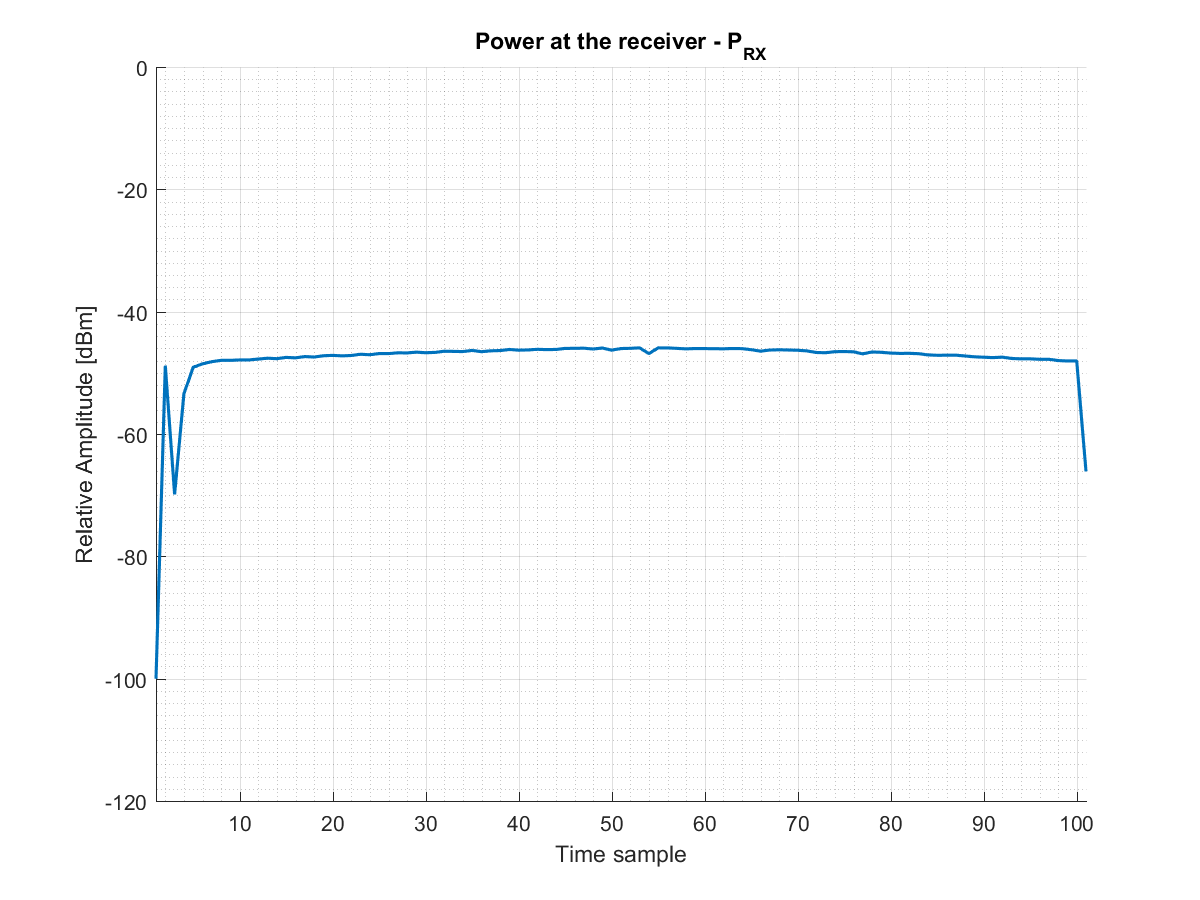
\includegraphics[scale=0.34]{figures/s1_pid_power.png}}
	\hfill
	\caption{UA Controllers}
	\label{fig:s1_power}
\end{figure}
